\subsection{Paquete 9: Panel de administración, gobernanza y moderación global}

    El paquete gestiona las funciones disciplinarias y la mediación en disputas dentro de la plataforma. Cualquier usuario puede denunciar comportamientos contrarios a las normas de convivencia, mientras que los administradores revisan chats notificados, resuelven quejas en bloque y sancionan infractores inhabilitando cuentas o retirando anuncios. La figura \ref{fig:dcu_moderacion} reúne los once casos de uso del módulo (CU76 a CU86).

\begin{figure}[H]
    \centering
    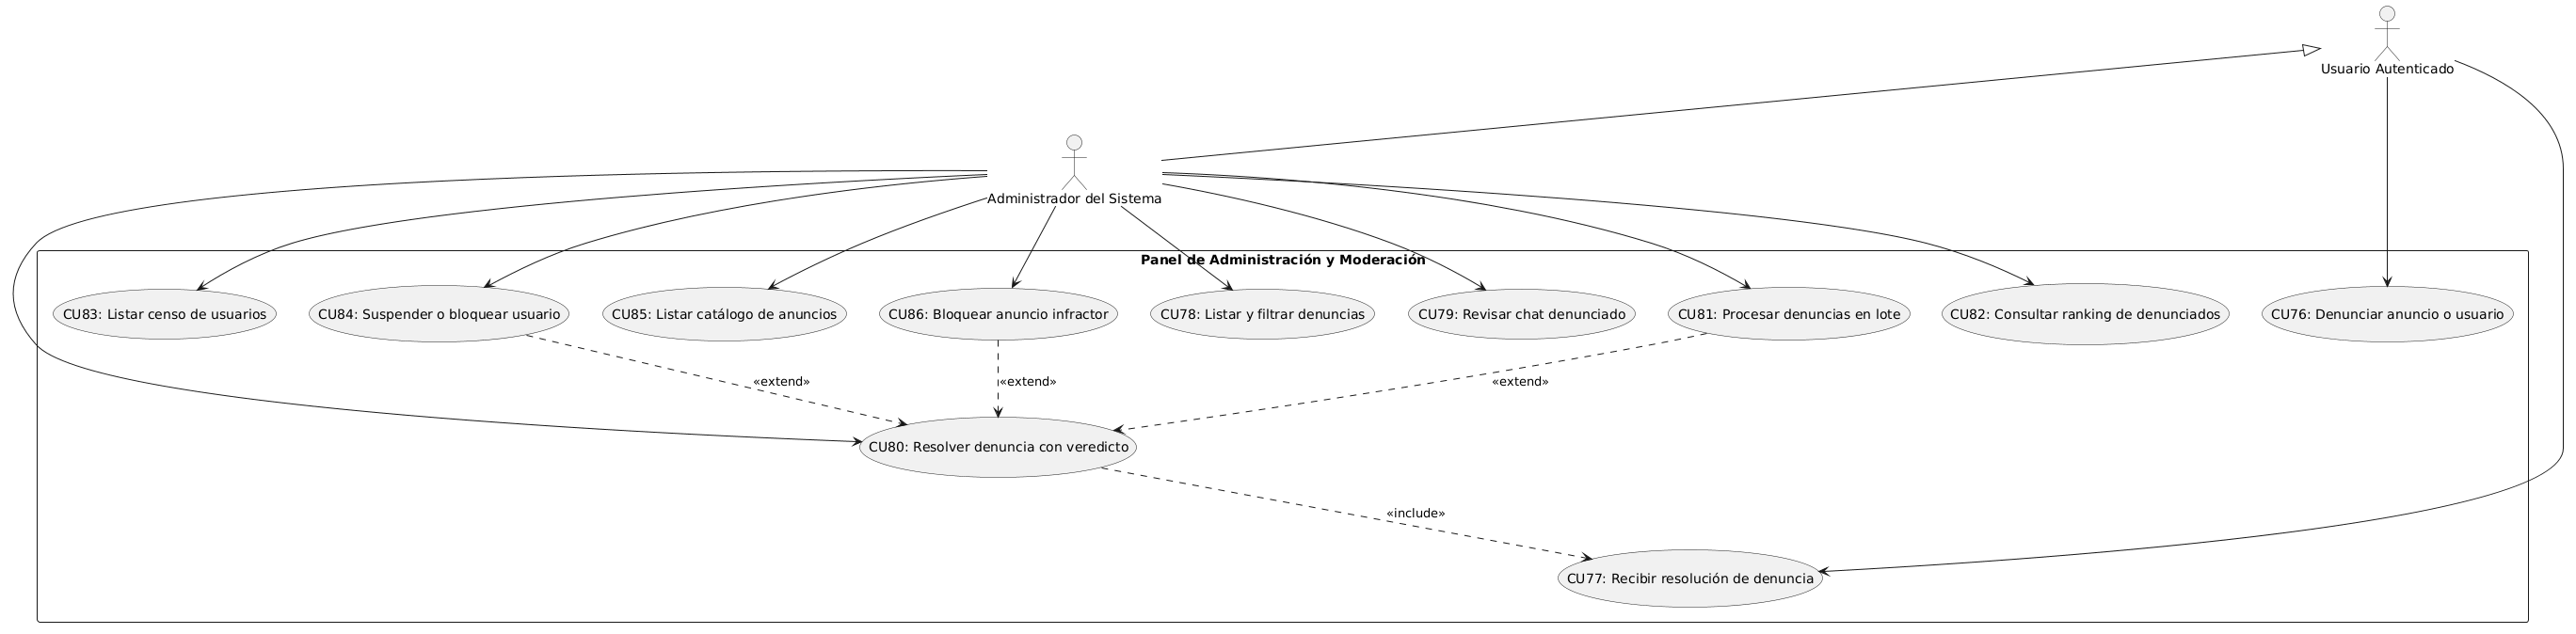
\includegraphics[width=0.88\textwidth]{AnalisisFuncional/img/dcu_moderacion.png}
    \caption{Diagrama de casos de uso de moderación y administración global}
    \label{fig:dcu_moderacion}
\end{figure}

    Las siguientes fichas estructuran las operaciones de moderación (CU76 a CU86):

\begin{table}[H]
\centering
\begin{tabular}{|p{3.2cm}|p{11.3cm}|}
\hline
\textbf{Caso de Uso} & \textbf{CU76: Denunciar anuncio, usuario o conversación} \\ \hline
\textbf{Actores} & Usuario Autenticado \\ \hline
\textbf{Descripción} & Remite una queja formal detallando una infracción sobre un contenido o conducta observada \\ \hline
\textbf{Precondiciones} & Estar autenticado y no haber denunciado previamente el mismo elemento si sigue en trámite \\ \hline
\textbf{Flujo básico} & 
1. El usuario pulsa sobre la opción de reporte presente en el anuncio, perfil o chat. \newline
2. El usuario selecciona la categoría del motivo y aporta una descripción justificativa. \newline
3. El backend registra la denuncia en estado pendiente dentro de la cola de moderación. \newline
4. El sistema confirma la recepción del reporte asignando un identificador de seguimiento. \\ \hline
\end{tabular}
\caption{Especificación del caso de uso CU76}
\label{tab:cu76}
\end{table}

\begin{table}[H]
\centering
\begin{tabular}{|p{3.2cm}|p{11.3cm}|}
\hline
\textbf{Caso de Uso} & \textbf{CU77: Recibir notificación de resolución de denuncia} \\ \hline
\textbf{Actores} & Usuario Autenticado \\ \hline
\textbf{Descripción} & Informa al usuario denunciante sobre el dictamen adoptado respecto a su notificación \\ \hline
\textbf{Precondiciones} & Haber interpuesto una denuncia que haya sido formalmente resuelta \\ \hline
\textbf{Flujo básico} & 
1. El sistema procesa el veredicto adoptado por el administrador sobre el expediente. \newline
2. El backend marca la denuncia con la confirmación de retroalimentación emitida. \newline
3. El sistema remite un aviso al panel de notificaciones del denunciante con el dictamen. \\ \hline
\end{tabular}
\caption{Especificación del caso de uso CU77}
\label{tab:cu77}
\end{table}

\begin{table}[H]
\centering
\begin{tabular}{|p{3.2cm}|p{11.3cm}|}
\hline
\textbf{Caso de Uso} & \textbf{CU78: Listar y filtrar cola global de denuncias} \\ \hline
\textbf{Actores} & Administrador del Sistema \\ \hline
\textbf{Descripción} & Despliega las quejas registradas permitiendo su clasificación por estado, severidad o tipo \\ \hline
\textbf{Precondiciones} & Disponer del rol de administración del sistema \\ \hline
\textbf{Flujo básico} & 
1. El administrador accede al panel de moderación global. \newline
2. El administrador aplica filtros por fecha, tipología del elemento o gravedad. \newline
3. El sistema recupera el listado paginado ordenado por orden cronológico y prioridad. \newline
4. La interfaz renderiza las tarjetas con el estado y los detalles preliminares del caso. \\ \hline
\end{tabular}
\caption{Especificación del caso de uso CU78}
\label{tab:cu78}
\end{table}

\begin{table}[H]
\centering
\begin{tabular}{|p{3.2cm}|p{11.3cm}|}
\hline
\textbf{Caso de Uso} & \textbf{CU79: Revisar historial de conversación denunciada} \\ \hline
\textbf{Actores} & Administrador del Sistema \\ \hline
\textbf{Descripción} & Audita de manera segura los mensajes intercambiados en un hilo objeto de investigación \\ \hline
\textbf{Precondiciones} & Que la denuncia corresponda formalmente a una infracción en el contexto del chat \\ \hline
\textbf{Flujo básico} & 
1. El administrador pulsa sobre el enlace de inspección dentro de la ficha del reporte. \newline
2. El sistema valida los permisos de auditoría y recupera los mensajes del canal. \newline
3. La interfaz presenta la secuencia íntegra de intervenciones para contrastar los hechos. \\ \hline
\end{tabular}
\caption{Especificación del caso de uso CU79}
\label{tab:cu79}
\end{table}

\begin{table}[H]
\centering
\begin{tabular}{|p{3.2cm}|p{11.3cm}|}
\hline
\textbf{Caso de Uso} & \textbf{CU80: Resolver denuncia individual con veredicto} \\ \hline
\textbf{Actores} & Administrador del Sistema \\ \hline
\textbf{Descripción} & Dictamina una queja asignando un estado de estimación o desestimación con notas técnicas \\ \hline
\textbf{Precondiciones} & Que el expediente de denuncia se encuentre en estado pendiente o en revisión \\ \hline
\textbf{Flujo básico} & 
1. El administrador introduce la justificación del veredicto y selecciona la resolución. \newline
2. El backend conmuta el estado de la denuncia a resuelta archivando el motivo del fallo. \newline
3. Se invoca de forma obligatoria la emisión de la notificación de retroalimentación al denunciante. \\ \hline
\end{tabular}
\caption{Especificación del caso de uso CU80}
\label{tab:cu80}
\end{table}

\begin{table}[H]
\centering
\begin{tabular}{|p{3.2cm}|p{11.3cm}|}
\hline
\textbf{Caso de Uso} & \textbf{CU81: Procesar denuncias en lote} \\ \hline
\textbf{Actores} & Administrador del Sistema \\ \hline
\textbf{Descripción} & Permite resolver conjuntamente múltiples denuncias vinculadas a un mismo infractor \\ \hline
\textbf{Precondiciones} & Existencia de al menos dos quejas pendientes asociadas a la misma entidad \\ \hline
\textbf{Flujo básico} & 
1. El administrador marca un grupo de denuncias acumuladas sobre un mismo elemento. \newline
2. El administrador define una resolución común y un veredicto unificado. \newline
3. Se extiende de forma reiterada la resolución individual con dictamen para cada expediente. \newline
4. El backend actualiza masivamente los registros dentro de una misma transacción. \\ \hline
\end{tabular}
\caption{Especificación del caso de uso CU81}
\label{tab:cu81}
\end{table}

\begin{table}[H]
\centering
\begin{tabular}{|p{3.2cm}|p{11.3cm}|}
\hline
\textbf{Caso de Uso} & \textbf{CU82: Consultar ranking de elementos más denunciados} \\ \hline
\textbf{Actores} & Administrador del Sistema \\ \hline
\textbf{Descripción} & Despliega métricas consolidadas sobre los usuarios y publicaciones con mayor tasa de reportes \\ \hline
\textbf{Precondiciones} & Disponer de credenciales activas de administrador \\ \hline
\textbf{Flujo básico} & 
1. El administrador accede al panel de métricas y tendencias de moderación. \newline
2. El sistema agrega la cantidad de reportes agrupados por identificador de entidad denunciada. \newline
3. La interfaz presenta una tabla ordenada descendentemente destacando a infractores recurrentes. \\ \hline
\end{tabular}
\caption{Especificación del caso de uso CU82}
\label{tab:cu82}
\end{table}

\begin{table}[H]
\centering
\begin{tabular}{|p{3.2cm}|p{11.3cm}|}
\hline
\textbf{Caso de Uso} & \textbf{CU83: Listar usuarios registrados con filtros} \\ \hline
\textbf{Actores} & Administrador del Sistema \\ \hline
\textbf{Descripción} & Muestra el censo global de cuentas en la plataforma permitiendo segmentar por estado o rol \\ \hline
\textbf{Precondiciones} & Estar autenticado con rol de administración \\ \hline
\textbf{Flujo básico} & 
1. El administrador entra en el módulo de gestión de usuarios del panel directivo. \newline
2. El administrador introduce un criterio de búsqueda como correo, nombre o estado disciplinario. \newline
3. El backend devuelve la lista paginada reflejando fechas de registro y avisos previos. \\ \hline
\end{tabular}
\caption{Especificación del caso de uso CU83}
\label{tab:cu83}
\end{table}

\begin{table}[H]
\centering
\begin{tabular}{|p{3.2cm}|p{11.3cm}|}
\hline
\textbf{Caso de Uso} & \textbf{CU84: Suspender o bloquear usuario de la plataforma} \\ \hline
\textbf{Actores} & Administrador del Sistema \\ \hline
\textbf{Descripción} & Inhabilita temporal o definitivamente el acceso al sistema de un infractor \\ \hline
\textbf{Precondiciones} & Que la cuenta a sancionar se encuentre actualmente en estado activo \\ \hline
\textbf{Flujo básico} & 
1. El administrador activa la sanción sobre el perfil del infractor especificando el motivo. \newline
2. Si la acción dimana de un informe disciplinario, se ejecuta de forma extendida sobre la resolución del reporte. \newline
3. El backend revoca de manera inmediata todos los tókenes JWT activos del usuario. \newline
4. El sistema bloquea los futuros intentos de autenticación impidiendo el acceso a la API. \\ \hline
\end{tabular}
\caption{Especificación del caso de uso CU84}
\label{tab:cu84}
\end{table}

\begin{table}[H]
\centering
\begin{tabular}{|p{3.2cm}|p{11.3cm}|}
\hline
\textbf{Caso de Uso} & \textbf{CU85: Listar catálogo global de anuncios} \\ \hline
\textbf{Actores} & Administrador del Sistema \\ \hline
\textbf{Descripción} & Examina la totalidad de los alojamientos registrados con independencia de su visibilidad \\ \hline
\textbf{Precondiciones} & Disponer de privilegios de administración \\ \hline
\textbf{Flujo básico} & 
1. El administrador accede a la auditoría del catálogo de propiedades. \newline
2. El sistema recupera los anuncios activos, pausados y bloqueados de todos los anfitriones. \newline
3. La interfaz permite consultar los importes, propietarios asociados e historiales de quejas. \\ \hline
\end{tabular}
\caption{Especificación del caso de uso CU85}
\label{tab:cu85}
\end{table}

\begin{table}[H]
\centering
\begin{tabular}{|p{3.2cm}|p{11.3cm}|}
\hline
\textbf{Caso de Uso} & \textbf{CU86: Bloquear o despublicar anuncio infractor} \\ \hline
\textbf{Actores} & Administrador del Sistema \\ \hline
\textbf{Descripción} & Retira una publicación del catálogo público por vulnerar las condiciones del servicio \\ \hline
\textbf{Precondiciones} & Que el anuncio figure en estado publicado o disponible \\ \hline
\textbf{Flujo básico} & 
1. El administrador selecciona la opción de bloqueo sobre la ficha del alojamiento infractor. \newline
2. Si procede de una denuncia, la medida se extiende sobre la resolución del reporte evaluado. \newline
3. El backend altera el estado de la publicación a bloqueada por moderación. \newline
4. El sistema purga la oferta de los resultados de búsqueda y del mapa interactivo. \\ \hline
\end{tabular}
\caption{Especificación del caso de uso CU86}
\label{tab:cu86}
\end{table}